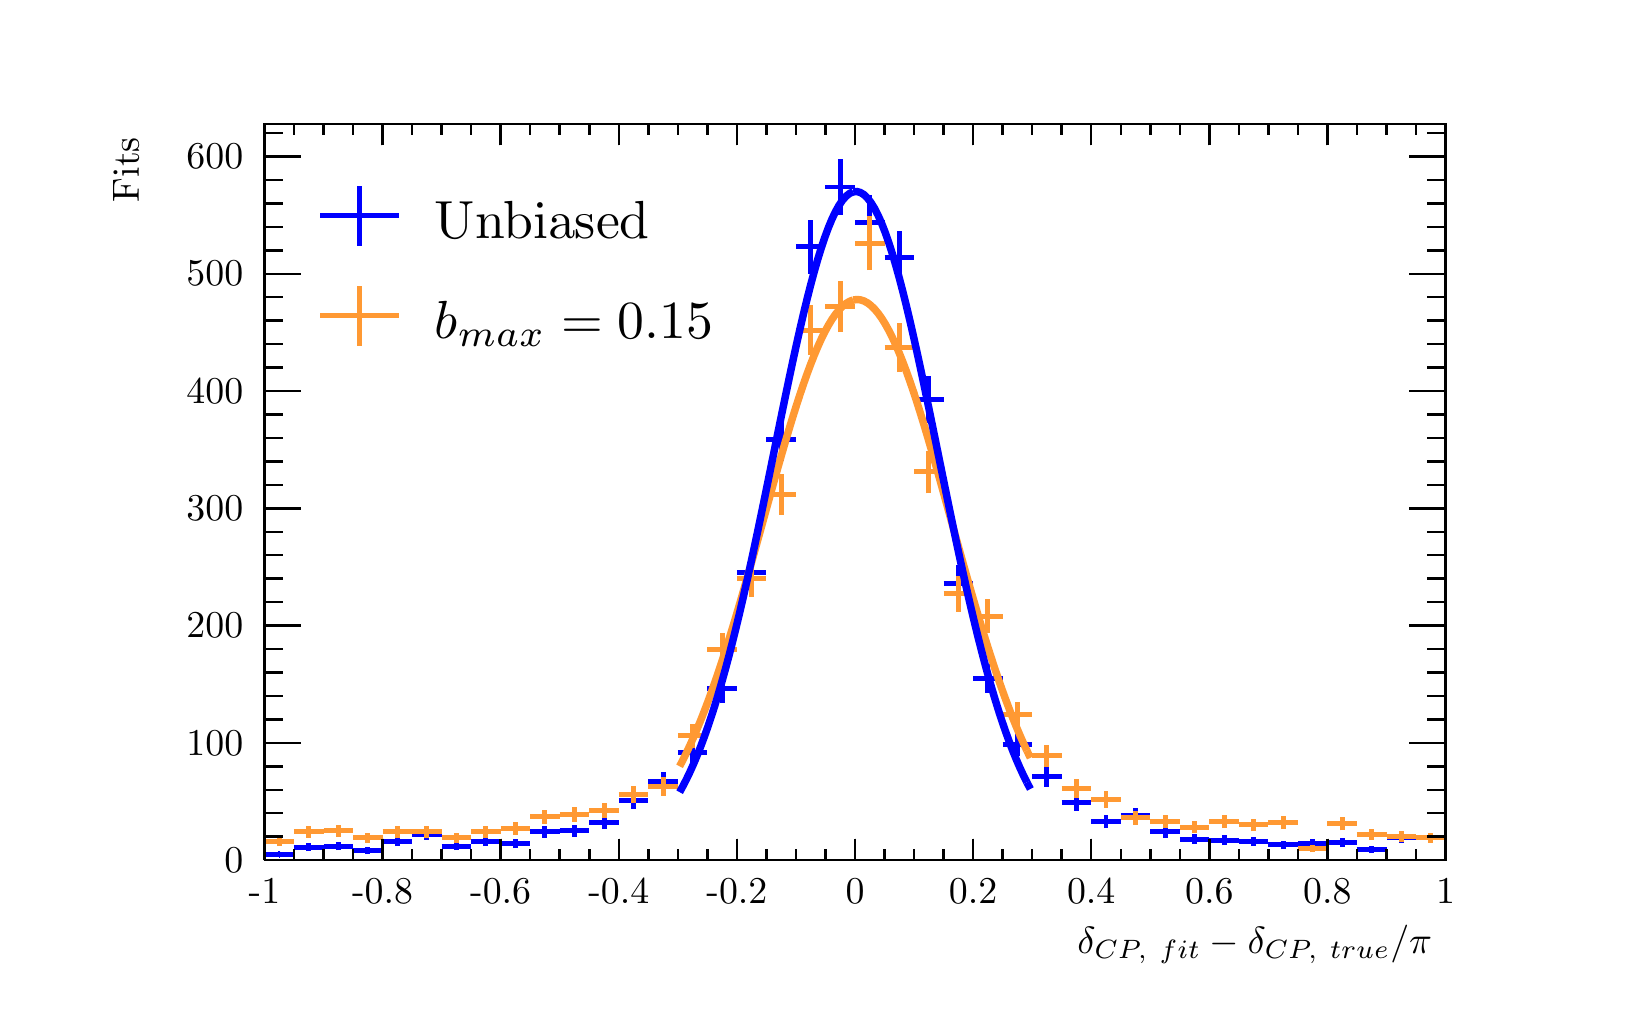
\begin{tikzpicture}
\pgfdeclareplotmark{cross} {
\pgfpathmoveto{\pgfpoint{-0.3\pgfplotmarksize}{\pgfplotmarksize}}
\pgfpathlineto{\pgfpoint{+0.3\pgfplotmarksize}{\pgfplotmarksize}}
\pgfpathlineto{\pgfpoint{+0.3\pgfplotmarksize}{0.3\pgfplotmarksize}}
\pgfpathlineto{\pgfpoint{+1\pgfplotmarksize}{0.3\pgfplotmarksize}}
\pgfpathlineto{\pgfpoint{+1\pgfplotmarksize}{-0.3\pgfplotmarksize}}
\pgfpathlineto{\pgfpoint{+0.3\pgfplotmarksize}{-0.3\pgfplotmarksize}}
\pgfpathlineto{\pgfpoint{+0.3\pgfplotmarksize}{-1.\pgfplotmarksize}}
\pgfpathlineto{\pgfpoint{-0.3\pgfplotmarksize}{-1.\pgfplotmarksize}}
\pgfpathlineto{\pgfpoint{-0.3\pgfplotmarksize}{-0.3\pgfplotmarksize}}
\pgfpathlineto{\pgfpoint{-1.\pgfplotmarksize}{-0.3\pgfplotmarksize}}
\pgfpathlineto{\pgfpoint{-1.\pgfplotmarksize}{0.3\pgfplotmarksize}}
\pgfpathlineto{\pgfpoint{-0.3\pgfplotmarksize}{0.3\pgfplotmarksize}}
\pgfpathclose
\pgfusepathqstroke
}
\pgfdeclareplotmark{cross*} {
\pgfpathmoveto{\pgfpoint{-0.3\pgfplotmarksize}{\pgfplotmarksize}}
\pgfpathlineto{\pgfpoint{+0.3\pgfplotmarksize}{\pgfplotmarksize}}
\pgfpathlineto{\pgfpoint{+0.3\pgfplotmarksize}{0.3\pgfplotmarksize}}
\pgfpathlineto{\pgfpoint{+1\pgfplotmarksize}{0.3\pgfplotmarksize}}
\pgfpathlineto{\pgfpoint{+1\pgfplotmarksize}{-0.3\pgfplotmarksize}}
\pgfpathlineto{\pgfpoint{+0.3\pgfplotmarksize}{-0.3\pgfplotmarksize}}
\pgfpathlineto{\pgfpoint{+0.3\pgfplotmarksize}{-1.\pgfplotmarksize}}
\pgfpathlineto{\pgfpoint{-0.3\pgfplotmarksize}{-1.\pgfplotmarksize}}
\pgfpathlineto{\pgfpoint{-0.3\pgfplotmarksize}{-0.3\pgfplotmarksize}}
\pgfpathlineto{\pgfpoint{-1.\pgfplotmarksize}{-0.3\pgfplotmarksize}}
\pgfpathlineto{\pgfpoint{-1.\pgfplotmarksize}{0.3\pgfplotmarksize}}
\pgfpathlineto{\pgfpoint{-0.3\pgfplotmarksize}{0.3\pgfplotmarksize}}
\pgfpathclose
\pgfusepathqfillstroke
}
\pgfdeclareplotmark{newstar} {
\pgfpathmoveto{\pgfqpoint{0pt}{\pgfplotmarksize}}
\pgfpathlineto{\pgfqpointpolar{44}{0.5\pgfplotmarksize}}
\pgfpathlineto{\pgfqpointpolar{18}{\pgfplotmarksize}}
\pgfpathlineto{\pgfqpointpolar{-20}{0.5\pgfplotmarksize}}
\pgfpathlineto{\pgfqpointpolar{-54}{\pgfplotmarksize}}
\pgfpathlineto{\pgfqpointpolar{-90}{0.5\pgfplotmarksize}}
\pgfpathlineto{\pgfqpointpolar{234}{\pgfplotmarksize}}
\pgfpathlineto{\pgfqpointpolar{198}{0.5\pgfplotmarksize}}
\pgfpathlineto{\pgfqpointpolar{162}{\pgfplotmarksize}}
\pgfpathlineto{\pgfqpointpolar{134}{0.5\pgfplotmarksize}}
\pgfpathclose
\pgfusepathqstroke
}
\pgfdeclareplotmark{newstar*} {
\pgfpathmoveto{\pgfqpoint{0pt}{\pgfplotmarksize}}
\pgfpathlineto{\pgfqpointpolar{44}{0.5\pgfplotmarksize}}
\pgfpathlineto{\pgfqpointpolar{18}{\pgfplotmarksize}}
\pgfpathlineto{\pgfqpointpolar{-20}{0.5\pgfplotmarksize}}
\pgfpathlineto{\pgfqpointpolar{-54}{\pgfplotmarksize}}
\pgfpathlineto{\pgfqpointpolar{-90}{0.5\pgfplotmarksize}}
\pgfpathlineto{\pgfqpointpolar{234}{\pgfplotmarksize}}
\pgfpathlineto{\pgfqpointpolar{198}{0.5\pgfplotmarksize}}
\pgfpathlineto{\pgfqpointpolar{162}{\pgfplotmarksize}}
\pgfpathlineto{\pgfqpointpolar{134}{0.5\pgfplotmarksize}}
\pgfpathclose
\pgfusepathqfillstroke
}
\definecolor{c}{rgb}{1,1,1};
\draw [color=c, fill=c] (0,0) rectangle (20,12.1438);
\draw [color=c, fill=c] (3,1.57869) rectangle (18,10.9294);
\definecolor{c}{rgb}{0,0,0};
\draw [c,line width=0.9] (3,1.57869) -- (3,10.9294) -- (18,10.9294) -- (18,1.57869) -- (3,1.57869);
\definecolor{c}{rgb}{1,1,1};
\draw [color=c, fill=c] (3,1.57869) rectangle (18,10.9294);
\definecolor{c}{rgb}{0,0,0};
\draw [c,line width=0.9] (3,1.57869) -- (3,10.9294) -- (18,10.9294) -- (18,1.57869) -- (3,1.57869);
\draw [c,line width=0.9] (3,1.57869) -- (18,1.57869);
\draw [c,line width=0.9] (3,1.85193) -- (3,1.57869);
\draw [c,line width=0.9] (3.375,1.71531) -- (3.375,1.57869);
\draw [c,line width=0.9] (3.75,1.71531) -- (3.75,1.57869);
\draw [c,line width=0.9] (4.125,1.71531) -- (4.125,1.57869);
\draw [c,line width=0.9] (4.5,1.85193) -- (4.5,1.57869);
\draw [c,line width=0.9] (4.875,1.71531) -- (4.875,1.57869);
\draw [c,line width=0.9] (5.25,1.71531) -- (5.25,1.57869);
\draw [c,line width=0.9] (5.625,1.71531) -- (5.625,1.57869);
\draw [c,line width=0.9] (6,1.85193) -- (6,1.57869);
\draw [c,line width=0.9] (6.375,1.71531) -- (6.375,1.57869);
\draw [c,line width=0.9] (6.75,1.71531) -- (6.75,1.57869);
\draw [c,line width=0.9] (7.125,1.71531) -- (7.125,1.57869);
\draw [c,line width=0.9] (7.5,1.85193) -- (7.5,1.57869);
\draw [c,line width=0.9] (7.875,1.71531) -- (7.875,1.57869);
\draw [c,line width=0.9] (8.25,1.71531) -- (8.25,1.57869);
\draw [c,line width=0.9] (8.625,1.71531) -- (8.625,1.57869);
\draw [c,line width=0.9] (9,1.85193) -- (9,1.57869);
\draw [c,line width=0.9] (9.375,1.71531) -- (9.375,1.57869);
\draw [c,line width=0.9] (9.75,1.71531) -- (9.75,1.57869);
\draw [c,line width=0.9] (10.125,1.71531) -- (10.125,1.57869);
\draw [c,line width=0.9] (10.5,1.85193) -- (10.5,1.57869);
\draw [c,line width=0.9] (10.875,1.71531) -- (10.875,1.57869);
\draw [c,line width=0.9] (11.25,1.71531) -- (11.25,1.57869);
\draw [c,line width=0.9] (11.625,1.71531) -- (11.625,1.57869);
\draw [c,line width=0.9] (12,1.85193) -- (12,1.57869);
\draw [c,line width=0.9] (12.375,1.71531) -- (12.375,1.57869);
\draw [c,line width=0.9] (12.75,1.71531) -- (12.75,1.57869);
\draw [c,line width=0.9] (13.125,1.71531) -- (13.125,1.57869);
\draw [c,line width=0.9] (13.5,1.85193) -- (13.5,1.57869);
\draw [c,line width=0.9] (13.875,1.71531) -- (13.875,1.57869);
\draw [c,line width=0.9] (14.25,1.71531) -- (14.25,1.57869);
\draw [c,line width=0.9] (14.625,1.71531) -- (14.625,1.57869);
\draw [c,line width=0.9] (15,1.85193) -- (15,1.57869);
\draw [c,line width=0.9] (15.375,1.71531) -- (15.375,1.57869);
\draw [c,line width=0.9] (15.75,1.71531) -- (15.75,1.57869);
\draw [c,line width=0.9] (16.125,1.71531) -- (16.125,1.57869);
\draw [c,line width=0.9] (16.5,1.85193) -- (16.5,1.57869);
\draw [c,line width=0.9] (16.875,1.71531) -- (16.875,1.57869);
\draw [c,line width=0.9] (17.25,1.71531) -- (17.25,1.57869);
\draw [c,line width=0.9] (17.625,1.71531) -- (17.625,1.57869);
\draw [c,line width=0.9] (18,1.85193) -- (18,1.57869);
\draw [c,line width=0.9] (3,1.85193) -- (3,1.57869);
\draw [c,line width=0.9] (18,1.85193) -- (18,1.57869);
\draw [anchor=base] (3,1.03222) node[scale=1.36851, color=c, rotate=0]{-1};
\draw [anchor=base] (4.5,1.03222) node[scale=1.36851, color=c, rotate=0]{-0.8};
\draw [anchor=base] (6,1.03222) node[scale=1.36851, color=c, rotate=0]{-0.6};
\draw [anchor=base] (7.5,1.03222) node[scale=1.36851, color=c, rotate=0]{-0.4};
\draw [anchor=base] (9,1.03222) node[scale=1.36851, color=c, rotate=0]{-0.2};
\draw [anchor=base] (10.5,1.03222) node[scale=1.36851, color=c, rotate=0]{0};
\draw [anchor=base] (12,1.03222) node[scale=1.36851, color=c, rotate=0]{0.2};
\draw [anchor=base] (13.5,1.03222) node[scale=1.36851, color=c, rotate=0]{0.4};
\draw [anchor=base] (15,1.03222) node[scale=1.36851, color=c, rotate=0]{0.6};
\draw [anchor=base] (16.5,1.03222) node[scale=1.36851, color=c, rotate=0]{0.8};
\draw [anchor=base] (18,1.03222) node[scale=1.36851, color=c, rotate=0]{1};
\draw [anchor= east] (18,0.510038) node[scale=1.36851, color=c, rotate=0]{$ \delta_{CP,~\text{fit}} - \delta_{CP,~\text{true}} / \pi$};
\draw [c,line width=0.9] (3,10.9294) -- (18,10.9294);
\draw [c,line width=0.9] (3,10.6562) -- (3,10.9294);
\draw [c,line width=0.9] (3.375,10.7928) -- (3.375,10.9294);
\draw [c,line width=0.9] (3.75,10.7928) -- (3.75,10.9294);
\draw [c,line width=0.9] (4.125,10.7928) -- (4.125,10.9294);
\draw [c,line width=0.9] (4.5,10.6562) -- (4.5,10.9294);
\draw [c,line width=0.9] (4.875,10.7928) -- (4.875,10.9294);
\draw [c,line width=0.9] (5.25,10.7928) -- (5.25,10.9294);
\draw [c,line width=0.9] (5.625,10.7928) -- (5.625,10.9294);
\draw [c,line width=0.9] (6,10.6562) -- (6,10.9294);
\draw [c,line width=0.9] (6.375,10.7928) -- (6.375,10.9294);
\draw [c,line width=0.9] (6.75,10.7928) -- (6.75,10.9294);
\draw [c,line width=0.9] (7.125,10.7928) -- (7.125,10.9294);
\draw [c,line width=0.9] (7.5,10.6562) -- (7.5,10.9294);
\draw [c,line width=0.9] (7.875,10.7928) -- (7.875,10.9294);
\draw [c,line width=0.9] (8.25,10.7928) -- (8.25,10.9294);
\draw [c,line width=0.9] (8.625,10.7928) -- (8.625,10.9294);
\draw [c,line width=0.9] (9,10.6562) -- (9,10.9294);
\draw [c,line width=0.9] (9.375,10.7928) -- (9.375,10.9294);
\draw [c,line width=0.9] (9.75,10.7928) -- (9.75,10.9294);
\draw [c,line width=0.9] (10.125,10.7928) -- (10.125,10.9294);
\draw [c,line width=0.9] (10.5,10.6562) -- (10.5,10.9294);
\draw [c,line width=0.9] (10.875,10.7928) -- (10.875,10.9294);
\draw [c,line width=0.9] (11.25,10.7928) -- (11.25,10.9294);
\draw [c,line width=0.9] (11.625,10.7928) -- (11.625,10.9294);
\draw [c,line width=0.9] (12,10.6562) -- (12,10.9294);
\draw [c,line width=0.9] (12.375,10.7928) -- (12.375,10.9294);
\draw [c,line width=0.9] (12.75,10.7928) -- (12.75,10.9294);
\draw [c,line width=0.9] (13.125,10.7928) -- (13.125,10.9294);
\draw [c,line width=0.9] (13.5,10.6562) -- (13.5,10.9294);
\draw [c,line width=0.9] (13.875,10.7928) -- (13.875,10.9294);
\draw [c,line width=0.9] (14.25,10.7928) -- (14.25,10.9294);
\draw [c,line width=0.9] (14.625,10.7928) -- (14.625,10.9294);
\draw [c,line width=0.9] (15,10.6562) -- (15,10.9294);
\draw [c,line width=0.9] (15.375,10.7928) -- (15.375,10.9294);
\draw [c,line width=0.9] (15.75,10.7928) -- (15.75,10.9294);
\draw [c,line width=0.9] (16.125,10.7928) -- (16.125,10.9294);
\draw [c,line width=0.9] (16.5,10.6562) -- (16.5,10.9294);
\draw [c,line width=0.9] (16.875,10.7928) -- (16.875,10.9294);
\draw [c,line width=0.9] (17.25,10.7928) -- (17.25,10.9294);
\draw [c,line width=0.9] (17.625,10.7928) -- (17.625,10.9294);
\draw [c,line width=0.9] (18,10.6562) -- (18,10.9294);
\draw [c,line width=0.9] (3,10.6562) -- (3,10.9294);
\draw [c,line width=0.9] (18,10.6562) -- (18,10.9294);
\draw [c,line width=0.9] (3,1.57869) -- (3,10.9294);
\draw [c,line width=0.9] (3.462,1.57869) -- (3,1.57869);
\draw [c,line width=0.9] (3.231,1.87655) -- (3,1.87655);
\draw [c,line width=0.9] (3.231,2.17441) -- (3,2.17441);
\draw [c,line width=0.9] (3.231,2.47227) -- (3,2.47227);
\draw [c,line width=0.9] (3.231,2.77014) -- (3,2.77014);
\draw [c,line width=0.9] (3.462,3.068) -- (3,3.068);
\draw [c,line width=0.9] (3.231,3.36586) -- (3,3.36586);
\draw [c,line width=0.9] (3.231,3.66372) -- (3,3.66372);
\draw [c,line width=0.9] (3.231,3.96158) -- (3,3.96158);
\draw [c,line width=0.9] (3.231,4.25944) -- (3,4.25944);
\draw [c,line width=0.9] (3.462,4.5573) -- (3,4.5573);
\draw [c,line width=0.9] (3.231,4.85517) -- (3,4.85517);
\draw [c,line width=0.9] (3.231,5.15303) -- (3,5.15303);
\draw [c,line width=0.9] (3.231,5.45089) -- (3,5.45089);
\draw [c,line width=0.9] (3.231,5.74875) -- (3,5.74875);
\draw [c,line width=0.9] (3.462,6.04661) -- (3,6.04661);
\draw [c,line width=0.9] (3.231,6.34447) -- (3,6.34447);
\draw [c,line width=0.9] (3.231,6.64233) -- (3,6.64233);
\draw [c,line width=0.9] (3.231,6.9402) -- (3,6.9402);
\draw [c,line width=0.9] (3.231,7.23806) -- (3,7.23806);
\draw [c,line width=0.9] (3.462,7.53592) -- (3,7.53592);
\draw [c,line width=0.9] (3.231,7.83378) -- (3,7.83378);
\draw [c,line width=0.9] (3.231,8.13164) -- (3,8.13164);
\draw [c,line width=0.9] (3.231,8.4295) -- (3,8.4295);
\draw [c,line width=0.9] (3.231,8.72736) -- (3,8.72736);
\draw [c,line width=0.9] (3.462,9.02523) -- (3,9.02523);
\draw [c,line width=0.9] (3.231,9.32309) -- (3,9.32309);
\draw [c,line width=0.9] (3.231,9.62095) -- (3,9.62095);
\draw [c,line width=0.9] (3.231,9.91881) -- (3,9.91881);
\draw [c,line width=0.9] (3.231,10.2167) -- (3,10.2167);
\draw [c,line width=0.9] (3.462,10.5145) -- (3,10.5145);
\draw [c,line width=0.9] (3.462,10.5145) -- (3,10.5145);
\draw [c,line width=0.9] (3.231,10.8124) -- (3,10.8124);
\draw [anchor= east] (2.9,1.57869) node[scale=1.36851, color=c, rotate=0]{0};
\draw [anchor= east] (2.9,3.068) node[scale=1.36851, color=c, rotate=0]{100};
\draw [anchor= east] (2.9,4.5573) node[scale=1.36851, color=c, rotate=0]{200};
\draw [anchor= east] (2.9,6.04661) node[scale=1.36851, color=c, rotate=0]{300};
\draw [anchor= east] (2.9,7.53592) node[scale=1.36851, color=c, rotate=0]{400};
\draw [anchor= east] (2.9,9.02523) node[scale=1.36851, color=c, rotate=0]{500};
\draw [anchor= east] (2.9,10.5145) node[scale=1.36851, color=c, rotate=0]{600};
\draw [anchor= east] (1.24,10.9294) node[scale=1.36851, color=c, rotate=90]{ Fits};
\draw [c,line width=0.9] (18,1.57869) -- (18,10.9294);
\draw [c,line width=0.9] (17.538,1.57869) -- (18,1.57869);
\draw [c,line width=0.9] (17.769,1.87655) -- (18,1.87655);
\draw [c,line width=0.9] (17.769,2.17441) -- (18,2.17441);
\draw [c,line width=0.9] (17.769,2.47227) -- (18,2.47227);
\draw [c,line width=0.9] (17.769,2.77014) -- (18,2.77014);
\draw [c,line width=0.9] (17.538,3.068) -- (18,3.068);
\draw [c,line width=0.9] (17.769,3.36586) -- (18,3.36586);
\draw [c,line width=0.9] (17.769,3.66372) -- (18,3.66372);
\draw [c,line width=0.9] (17.769,3.96158) -- (18,3.96158);
\draw [c,line width=0.9] (17.769,4.25944) -- (18,4.25944);
\draw [c,line width=0.9] (17.538,4.5573) -- (18,4.5573);
\draw [c,line width=0.9] (17.769,4.85517) -- (18,4.85517);
\draw [c,line width=0.9] (17.769,5.15303) -- (18,5.15303);
\draw [c,line width=0.9] (17.769,5.45089) -- (18,5.45089);
\draw [c,line width=0.9] (17.769,5.74875) -- (18,5.74875);
\draw [c,line width=0.9] (17.538,6.04661) -- (18,6.04661);
\draw [c,line width=0.9] (17.769,6.34447) -- (18,6.34447);
\draw [c,line width=0.9] (17.769,6.64233) -- (18,6.64233);
\draw [c,line width=0.9] (17.769,6.9402) -- (18,6.9402);
\draw [c,line width=0.9] (17.769,7.23806) -- (18,7.23806);
\draw [c,line width=0.9] (17.538,7.53592) -- (18,7.53592);
\draw [c,line width=0.9] (17.769,7.83378) -- (18,7.83378);
\draw [c,line width=0.9] (17.769,8.13164) -- (18,8.13164);
\draw [c,line width=0.9] (17.769,8.4295) -- (18,8.4295);
\draw [c,line width=0.9] (17.769,8.72736) -- (18,8.72736);
\draw [c,line width=0.9] (17.538,9.02523) -- (18,9.02523);
\draw [c,line width=0.9] (17.769,9.32309) -- (18,9.32309);
\draw [c,line width=0.9] (17.769,9.62095) -- (18,9.62095);
\draw [c,line width=0.9] (17.769,9.91881) -- (18,9.91881);
\draw [c,line width=0.9] (17.769,10.2167) -- (18,10.2167);
\draw [c,line width=0.9] (17.538,10.5145) -- (18,10.5145);
\draw [c,line width=0.9] (17.538,10.5145) -- (18,10.5145);
\draw [c,line width=0.9] (17.769,10.8124) -- (18,10.8124);
\definecolor{c}{rgb}{0,0,1};
\draw [c,line width=1.8] (3.1875,1.61985) -- (3.1875,1.65316);
\draw [c,line width=1.8] (3.1875,1.65316) -- (3.1875,1.68646);
\draw [c,line width=1.8] (3,1.65316) -- (3.1875,1.65316);
\draw [c,line width=1.8] (3.1875,1.65316) -- (3.375,1.65316);
\foreach \P in {(3.1875,1.65316)}{\draw[mark options={color=c,fill=c},mark size=2.402402pt, line width=0.000000pt, mark=*,mark size=1pt] plot coordinates {\P};}
\draw [c,line width=1.8] (3.5625,1.69312) -- (3.5625,1.74251);
\draw [c,line width=1.8] (3.5625,1.74251) -- (3.5625,1.79191);
\draw [c,line width=1.8] (3.375,1.74251) -- (3.5625,1.74251);
\draw [c,line width=1.8] (3.5625,1.74251) -- (3.75,1.74251);
\foreach \P in {(3.5625,1.74251)}{\draw[mark options={color=c,fill=c},mark size=2.402402pt, line width=0.000000pt, mark=*,mark size=1pt] plot coordinates {\P};}
\draw [c,line width=1.8] (3.9375,1.70582) -- (3.9375,1.75741);
\draw [c,line width=1.8] (3.9375,1.75741) -- (3.9375,1.809);
\draw [c,line width=1.8] (3.75,1.75741) -- (3.9375,1.75741);
\draw [c,line width=1.8] (3.9375,1.75741) -- (4.125,1.75741);
\foreach \P in {(3.9375,1.75741)}{\draw[mark options={color=c,fill=c},mark size=2.402402pt, line width=0.000000pt, mark=*,mark size=1pt] plot coordinates {\P};}
\draw [c,line width=1.8] (4.3125,1.65571) -- (4.3125,1.69784);
\draw [c,line width=1.8] (4.3125,1.69784) -- (4.3125,1.73996);
\draw [c,line width=1.8] (4.125,1.69784) -- (4.3125,1.69784);
\draw [c,line width=1.8] (4.3125,1.69784) -- (4.5,1.69784);
\foreach \P in {(4.3125,1.69784)}{\draw[mark options={color=c,fill=c},mark size=2.402402pt, line width=0.000000pt, mark=*,mark size=1pt] plot coordinates {\P};}
\draw [c,line width=1.8] (4.6875,1.75741) -- (4.6875,1.81698);
\draw [c,line width=1.8] (4.6875,1.81698) -- (4.6875,1.87655);
\draw [c,line width=1.8] (4.5,1.81698) -- (4.6875,1.81698);
\draw [c,line width=1.8] (4.6875,1.81698) -- (4.875,1.81698);
\foreach \P in {(4.6875,1.81698)}{\draw[mark options={color=c,fill=c},mark size=2.402402pt, line width=0.000000pt, mark=*,mark size=1pt] plot coordinates {\P};}
\draw [c,line width=1.8] (5.0625,1.83648) -- (5.0625,1.90634);
\draw [c,line width=1.8] (5.0625,1.90634) -- (5.0625,1.97619);
\draw [c,line width=1.8] (4.875,1.90634) -- (5.0625,1.90634);
\draw [c,line width=1.8] (5.0625,1.90634) -- (5.25,1.90634);
\foreach \P in {(5.0625,1.90634)}{\draw[mark options={color=c,fill=c},mark size=2.402402pt, line width=0.000000pt, mark=*,mark size=1pt] plot coordinates {\P};}
\draw [c,line width=1.8] (5.4375,1.70582) -- (5.4375,1.75741);
\draw [c,line width=1.8] (5.4375,1.75741) -- (5.4375,1.809);
\draw [c,line width=1.8] (5.25,1.75741) -- (5.4375,1.75741);
\draw [c,line width=1.8] (5.4375,1.75741) -- (5.625,1.75741);
\foreach \P in {(5.4375,1.75741)}{\draw[mark options={color=c,fill=c},mark size=2.402402pt, line width=0.000000pt, mark=*,mark size=1pt] plot coordinates {\P};}
\draw [c,line width=1.8] (5.8125,1.75741) -- (5.8125,1.81698);
\draw [c,line width=1.8] (5.8125,1.81698) -- (5.8125,1.87655);
\draw [c,line width=1.8] (5.625,1.81698) -- (5.8125,1.81698);
\draw [c,line width=1.8] (5.8125,1.81698) -- (6,1.81698);
\foreach \P in {(5.8125,1.81698)}{\draw[mark options={color=c,fill=c},mark size=2.402402pt, line width=0.000000pt, mark=*,mark size=1pt] plot coordinates {\P};}
\draw [c,line width=1.8] (6.1875,1.73147) -- (6.1875,1.78719);
\draw [c,line width=1.8] (6.1875,1.78719) -- (6.1875,1.84292);
\draw [c,line width=1.8] (6,1.78719) -- (6.1875,1.78719);
\draw [c,line width=1.8] (6.1875,1.78719) -- (6.375,1.78719);
\foreach \P in {(6.1875,1.78719)}{\draw[mark options={color=c,fill=c},mark size=2.402402pt, line width=0.000000pt, mark=*,mark size=1pt] plot coordinates {\P};}
\draw [c,line width=1.8] (6.5625,1.86316) -- (6.5625,1.93612);
\draw [c,line width=1.8] (6.5625,1.93612) -- (6.5625,2.00909);
\draw [c,line width=1.8] (6.375,1.93612) -- (6.5625,1.93612);
\draw [c,line width=1.8] (6.5625,1.93612) -- (6.75,1.93612);
\foreach \P in {(6.5625,1.93612)}{\draw[mark options={color=c,fill=c},mark size=2.402402pt, line width=0.000000pt, mark=*,mark size=1pt] plot coordinates {\P};}
\draw [c,line width=1.8] (6.9375,1.87655) -- (6.9375,1.95102);
\draw [c,line width=1.8] (6.9375,1.95102) -- (6.9375,2.02548);
\draw [c,line width=1.8] (6.75,1.95102) -- (6.9375,1.95102);
\draw [c,line width=1.8] (6.9375,1.95102) -- (7.125,1.95102);
\foreach \P in {(6.9375,1.95102)}{\draw[mark options={color=c,fill=c},mark size=2.402402pt, line width=0.000000pt, mark=*,mark size=1pt] plot coordinates {\P};}
\draw [c,line width=1.8] (7.3125,1.97102) -- (7.3125,2.05527);
\draw [c,line width=1.8] (7.3125,2.05527) -- (7.3125,2.13952);
\draw [c,line width=1.8] (7.125,2.05527) -- (7.3125,2.05527);
\draw [c,line width=1.8] (7.3125,2.05527) -- (7.5,2.05527);
\foreach \P in {(7.3125,2.05527)}{\draw[mark options={color=c,fill=c},mark size=2.402402pt, line width=0.000000pt, mark=*,mark size=1pt] plot coordinates {\P};}
\draw [c,line width=1.8] (7.6875,2.23188) -- (7.6875,2.33824);
\draw [c,line width=1.8] (7.6875,2.33824) -- (7.6875,2.44459);
\draw [c,line width=1.8] (7.5,2.33824) -- (7.6875,2.33824);
\draw [c,line width=1.8] (7.6875,2.33824) -- (7.875,2.33824);
\foreach \P in {(7.6875,2.33824)}{\draw[mark options={color=c,fill=c},mark size=2.402402pt, line width=0.000000pt, mark=*,mark size=1pt] plot coordinates {\P};}
\draw [c,line width=1.8] (8.0625,2.45462) -- (8.0625,2.57653);
\draw [c,line width=1.8] (8.0625,2.57653) -- (8.0625,2.69843);
\draw [c,line width=1.8] (7.875,2.57653) -- (8.0625,2.57653);
\draw [c,line width=1.8] (8.0625,2.57653) -- (8.25,2.57653);
\foreach \P in {(8.0625,2.57653)}{\draw[mark options={color=c,fill=c},mark size=2.402402pt, line width=0.000000pt, mark=*,mark size=1pt] plot coordinates {\P};}
\draw [c,line width=1.8] (8.4375,2.806) -- (8.4375,2.94885);
\draw [c,line width=1.8] (8.4375,2.94885) -- (8.4375,3.0917);
\draw [c,line width=1.8] (8.25,2.94885) -- (8.4375,2.94885);
\draw [c,line width=1.8] (8.4375,2.94885) -- (8.625,2.94885);
\foreach \P in {(8.4375,2.94885)}{\draw[mark options={color=c,fill=c},mark size=2.402402pt, line width=0.000000pt, mark=*,mark size=1pt] plot coordinates {\P};}
\draw [c,line width=1.8] (8.8125,3.57313) -- (8.8125,3.75308);
\draw [c,line width=1.8] (8.8125,3.75308) -- (8.8125,3.93303);
\draw [c,line width=1.8] (8.625,3.75308) -- (8.8125,3.75308);
\draw [c,line width=1.8] (8.8125,3.75308) -- (9,3.75308);
\foreach \P in {(8.8125,3.75308)}{\draw[mark options={color=c,fill=c},mark size=2.402402pt, line width=0.000000pt, mark=*,mark size=1pt] plot coordinates {\P};}
\draw [c,line width=1.8] (9.1875,4.99438) -- (9.1875,5.22749);
\draw [c,line width=1.8] (9.1875,5.22749) -- (9.1875,5.46061);
\draw [c,line width=1.8] (9,5.22749) -- (9.1875,5.22749);
\draw [c,line width=1.8] (9.1875,5.22749) -- (9.375,5.22749);
\foreach \P in {(9.1875,5.22749)}{\draw[mark options={color=c,fill=c},mark size=2.402402pt, line width=0.000000pt, mark=*,mark size=1pt] plot coordinates {\P};}
\draw [c,line width=1.8] (9.5625,6.64312) -- (9.5625,6.9253);
\draw [c,line width=1.8] (9.5625,6.9253) -- (9.5625,7.20749);
\draw [c,line width=1.8] (9.375,6.9253) -- (9.5625,6.9253);
\draw [c,line width=1.8] (9.5625,6.9253) -- (9.75,6.9253);
\foreach \P in {(9.5625,6.9253)}{\draw[mark options={color=c,fill=c},mark size=2.402402pt, line width=0.000000pt, mark=*,mark size=1pt] plot coordinates {\P};}
\draw [c,line width=1.8] (9.9375,9.02717) -- (9.9375,9.36777);
\draw [c,line width=1.8] (9.9375,9.36777) -- (9.9375,9.70836);
\draw [c,line width=1.8] (9.75,9.36777) -- (9.9375,9.36777);
\draw [c,line width=1.8] (9.9375,9.36777) -- (10.125,9.36777);
\foreach \P in {(9.9375,9.36777)}{\draw[mark options={color=c,fill=c},mark size=2.402402pt, line width=0.000000pt, mark=*,mark size=1pt] plot coordinates {\P};}
\draw [c,line width=1.8] (10.3125,9.7705) -- (10.3125,10.1273);
\draw [c,line width=1.8] (10.3125,10.1273) -- (10.3125,10.4841);
\draw [c,line width=1.8] (10.125,10.1273) -- (10.3125,10.1273);
\draw [c,line width=1.8] (10.3125,10.1273) -- (10.5,10.1273);
\foreach \P in {(10.3125,10.1273)}{\draw[mark options={color=c,fill=c},mark size=2.402402pt, line width=0.000000pt, mark=*,mark size=1pt] plot coordinates {\P};}
\draw [c,line width=1.8] (10.6875,9.33316) -- (10.6875,9.68052);
\draw [c,line width=1.8] (10.6875,9.68052) -- (10.6875,10.0279);
\draw [c,line width=1.8] (10.5,9.68052) -- (10.6875,9.68052);
\draw [c,line width=1.8] (10.6875,9.68052) -- (10.875,9.68052);
\foreach \P in {(10.6875,9.68052)}{\draw[mark options={color=c,fill=c},mark size=2.402402pt, line width=0.000000pt, mark=*,mark size=1pt] plot coordinates {\P};}
\draw [c,line width=1.8] (11.0625,8.89608) -- (11.0625,9.23373);
\draw [c,line width=1.8] (11.0625,9.23373) -- (11.0625,9.57138);
\draw [c,line width=1.8] (10.875,9.23373) -- (11.0625,9.23373);
\draw [c,line width=1.8] (11.0625,9.23373) -- (11.25,9.23373);
\foreach \P in {(11.0625,9.23373)}{\draw[mark options={color=c,fill=c},mark size=2.402402pt, line width=0.000000pt, mark=*,mark size=1pt] plot coordinates {\P};}
\draw [c,line width=1.8] (11.4375,7.13642) -- (11.4375,7.43167);
\draw [c,line width=1.8] (11.4375,7.43167) -- (11.4375,7.72691);
\draw [c,line width=1.8] (11.25,7.43167) -- (11.4375,7.43167);
\draw [c,line width=1.8] (11.4375,7.43167) -- (11.625,7.43167);
\foreach \P in {(11.4375,7.43167)}{\draw[mark options={color=c,fill=c},mark size=2.402402pt, line width=0.000000pt, mark=*,mark size=1pt] plot coordinates {\P};}
\draw [c,line width=1.8] (11.8125,4.86466) -- (11.8125,5.09345);
\draw [c,line width=1.8] (11.8125,5.09345) -- (11.8125,5.32225);
\draw [c,line width=1.8] (11.625,5.09345) -- (11.8125,5.09345);
\draw [c,line width=1.8] (11.8125,5.09345) -- (12,5.09345);
\foreach \P in {(11.8125,5.09345)}{\draw[mark options={color=c,fill=c},mark size=2.402402pt, line width=0.000000pt, mark=*,mark size=1pt] plot coordinates {\P};}
\draw [c,line width=1.8] (12.1875,3.7017) -- (12.1875,3.88712);
\draw [c,line width=1.8] (12.1875,3.88712) -- (12.1875,4.07253);
\draw [c,line width=1.8] (12,3.88712) -- (12.1875,3.88712);
\draw [c,line width=1.8] (12.1875,3.88712) -- (12.375,3.88712);
\foreach \P in {(12.1875,3.88712)}{\draw[mark options={color=c,fill=c},mark size=2.402402pt, line width=0.000000pt, mark=*,mark size=1pt] plot coordinates {\P};}
\draw [c,line width=1.8] (12.5625,2.90492) -- (12.5625,3.0531);
\draw [c,line width=1.8] (12.5625,3.0531) -- (12.5625,3.20129);
\draw [c,line width=1.8] (12.375,3.0531) -- (12.5625,3.0531);
\draw [c,line width=1.8] (12.5625,3.0531) -- (12.75,3.0531);
\foreach \P in {(12.5625,3.0531)}{\draw[mark options={color=c,fill=c},mark size=2.402402pt, line width=0.000000pt, mark=*,mark size=1pt] plot coordinates {\P};}
\draw [c,line width=1.8] (12.9375,2.51061) -- (12.9375,2.6361);
\draw [c,line width=1.8] (12.9375,2.6361) -- (12.9375,2.76159);
\draw [c,line width=1.8] (12.75,2.6361) -- (12.9375,2.6361);
\draw [c,line width=1.8] (12.9375,2.6361) -- (13.125,2.6361);
\foreach \P in {(12.9375,2.6361)}{\draw[mark options={color=c,fill=c},mark size=2.402402pt, line width=0.000000pt, mark=*,mark size=1pt] plot coordinates {\P};}
\draw [c,line width=1.8] (13.3125,2.2042) -- (13.3125,2.30845);
\draw [c,line width=1.8] (13.3125,2.30845) -- (13.3125,2.4127);
\draw [c,line width=1.8] (13.125,2.30845) -- (13.3125,2.30845);
\draw [c,line width=1.8] (13.3125,2.30845) -- (13.5,2.30845);
\foreach \P in {(13.3125,2.30845)}{\draw[mark options={color=c,fill=c},mark size=2.402402pt, line width=0.000000pt, mark=*,mark size=1pt] plot coordinates {\P};}
\draw [c,line width=1.8] (13.6875,1.98461) -- (13.6875,2.07016);
\draw [c,line width=1.8] (13.6875,2.07016) -- (13.6875,2.15572);
\draw [c,line width=1.8] (13.5,2.07016) -- (13.6875,2.07016);
\draw [c,line width=1.8] (13.6875,2.07016) -- (13.875,2.07016);
\foreach \P in {(13.6875,2.07016)}{\draw[mark options={color=c,fill=c},mark size=2.402402pt, line width=0.000000pt, mark=*,mark size=1pt] plot coordinates {\P};}
\draw [c,line width=1.8] (14.0625,2.05282) -- (14.0625,2.14463);
\draw [c,line width=1.8] (14.0625,2.14463) -- (14.0625,2.23643);
\draw [c,line width=1.8] (13.875,2.14463) -- (14.0625,2.14463);
\draw [c,line width=1.8] (14.0625,2.14463) -- (14.25,2.14463);
\foreach \P in {(14.0625,2.14463)}{\draw[mark options={color=c,fill=c},mark size=2.402402pt, line width=0.000000pt, mark=*,mark size=1pt] plot coordinates {\P};}
\draw [c,line width=1.8] (14.4375,1.86316) -- (14.4375,1.93612);
\draw [c,line width=1.8] (14.4375,1.93612) -- (14.4375,2.00909);
\draw [c,line width=1.8] (14.25,1.93612) -- (14.4375,1.93612);
\draw [c,line width=1.8] (14.4375,1.93612) -- (14.625,1.93612);
\foreach \P in {(14.4375,1.93612)}{\draw[mark options={color=c,fill=c},mark size=2.402402pt, line width=0.000000pt, mark=*,mark size=1pt] plot coordinates {\P};}
\draw [c,line width=1.8] (14.8125,1.78358) -- (14.8125,1.84677);
\draw [c,line width=1.8] (14.8125,1.84677) -- (14.8125,1.90995);
\draw [c,line width=1.8] (14.625,1.84677) -- (14.8125,1.84677);
\draw [c,line width=1.8] (14.8125,1.84677) -- (15,1.84677);
\foreach \P in {(14.8125,1.84677)}{\draw[mark options={color=c,fill=c},mark size=2.402402pt, line width=0.000000pt, mark=*,mark size=1pt] plot coordinates {\P};}
\draw [c,line width=1.8] (15.1875,1.77047) -- (15.1875,1.83187);
\draw [c,line width=1.8] (15.1875,1.83187) -- (15.1875,1.89328);
\draw [c,line width=1.8] (15,1.83187) -- (15.1875,1.83187);
\draw [c,line width=1.8] (15.1875,1.83187) -- (15.375,1.83187);
\foreach \P in {(15.1875,1.83187)}{\draw[mark options={color=c,fill=c},mark size=2.402402pt, line width=0.000000pt, mark=*,mark size=1pt] plot coordinates {\P};}
\draw [c,line width=1.8] (15.5625,1.75741) -- (15.5625,1.81698);
\draw [c,line width=1.8] (15.5625,1.81698) -- (15.5625,1.87655);
\draw [c,line width=1.8] (15.375,1.81698) -- (15.5625,1.81698);
\draw [c,line width=1.8] (15.5625,1.81698) -- (15.75,1.81698);
\foreach \P in {(15.5625,1.81698)}{\draw[mark options={color=c,fill=c},mark size=2.402402pt, line width=0.000000pt, mark=*,mark size=1pt] plot coordinates {\P};}
\draw [c,line width=1.8] (15.9375,1.7186) -- (15.9375,1.7723);
\draw [c,line width=1.8] (15.9375,1.7723) -- (15.9375,1.826);
\draw [c,line width=1.8] (15.75,1.7723) -- (15.9375,1.7723);
\draw [c,line width=1.8] (15.9375,1.7723) -- (16.125,1.7723);
\foreach \P in {(15.9375,1.7723)}{\draw[mark options={color=c,fill=c},mark size=2.402402pt, line width=0.000000pt, mark=*,mark size=1pt] plot coordinates {\P};}
\draw [c,line width=1.8] (16.3125,1.73147) -- (16.3125,1.78719);
\draw [c,line width=1.8] (16.3125,1.78719) -- (16.3125,1.84292);
\draw [c,line width=1.8] (16.125,1.78719) -- (16.3125,1.78719);
\draw [c,line width=1.8] (16.3125,1.78719) -- (16.5,1.78719);
\foreach \P in {(16.3125,1.78719)}{\draw[mark options={color=c,fill=c},mark size=2.402402pt, line width=0.000000pt, mark=*,mark size=1pt] plot coordinates {\P};}
\draw [c,line width=1.8] (16.6875,1.74441) -- (16.6875,1.80209);
\draw [c,line width=1.8] (16.6875,1.80209) -- (16.6875,1.85977);
\draw [c,line width=1.8] (16.5,1.80209) -- (16.6875,1.80209);
\draw [c,line width=1.8] (16.6875,1.80209) -- (16.875,1.80209);
\foreach \P in {(16.6875,1.80209)}{\draw[mark options={color=c,fill=c},mark size=2.402402pt, line width=0.000000pt, mark=*,mark size=1pt] plot coordinates {\P};}
\draw [c,line width=1.8] (17.0625,1.66805) -- (17.0625,1.71273);
\draw [c,line width=1.8] (17.0625,1.71273) -- (17.0625,1.75741);
\draw [c,line width=1.8] (16.875,1.71273) -- (17.0625,1.71273);
\draw [c,line width=1.8] (17.0625,1.71273) -- (17.25,1.71273);
\foreach \P in {(17.0625,1.71273)}{\draw[mark options={color=c,fill=c},mark size=2.402402pt, line width=0.000000pt, mark=*,mark size=1pt] plot coordinates {\P};}
\draw [c,line width=1.8] (17.4375,1.79674) -- (17.4375,1.86166);
\draw [c,line width=1.8] (17.4375,1.86166) -- (17.4375,1.92658);
\draw [c,line width=1.8] (17.25,1.86166) -- (17.4375,1.86166);
\draw [c,line width=1.8] (17.4375,1.86166) -- (17.625,1.86166);
\foreach \P in {(17.4375,1.86166)}{\draw[mark options={color=c,fill=c},mark size=2.402402pt, line width=0.000000pt, mark=*,mark size=1pt] plot coordinates {\P};}
\draw [c,line width=1.8] (17.8125,1.79674) -- (17.8125,1.86166);
\draw [c,line width=1.8] (17.8125,1.86166) -- (17.8125,1.92658);
\draw [c,line width=1.8] (17.625,1.86166) -- (17.8125,1.86166);
\draw [c,line width=1.8] (17.8125,1.86166) -- (18,1.86166);
\foreach \P in {(17.8125,1.86166)}{\draw[mark options={color=c,fill=c},mark size=2.402402pt, line width=0.000000pt, mark=*,mark size=1pt] plot coordinates {\P};}
\definecolor{c}{rgb}{1,0.6,0.2};
\draw [c,line width=1.8] (3.1875,1.75741) -- (3.1875,1.81698);
\draw [c,line width=1.8] (3.1875,1.81698) -- (3.1875,1.87655);
\draw [c,line width=1.8] (3,1.81698) -- (3.1875,1.81698);
\draw [c,line width=1.8] (3.1875,1.81698) -- (3.375,1.81698);
\foreach \P in {(3.1875,1.81698)}{\draw[mark options={color=c,fill=c},mark size=2.402402pt, line width=0.000000pt, mark=*,mark size=1pt] plot coordinates {\P};}
\draw [c,line width=1.8] (3.5625,1.86316) -- (3.5625,1.93612);
\draw [c,line width=1.8] (3.5625,1.93612) -- (3.5625,2.00909);
\draw [c,line width=1.8] (3.375,1.93612) -- (3.5625,1.93612);
\draw [c,line width=1.8] (3.5625,1.93612) -- (3.75,1.93612);
\foreach \P in {(3.5625,1.93612)}{\draw[mark options={color=c,fill=c},mark size=2.402402pt, line width=0.000000pt, mark=*,mark size=1pt] plot coordinates {\P};}
\draw [c,line width=1.8] (3.9375,1.87655) -- (3.9375,1.95102);
\draw [c,line width=1.8] (3.9375,1.95102) -- (3.9375,2.02548);
\draw [c,line width=1.8] (3.75,1.95102) -- (3.9375,1.95102);
\draw [c,line width=1.8] (3.9375,1.95102) -- (4.125,1.95102);
\foreach \P in {(3.9375,1.95102)}{\draw[mark options={color=c,fill=c},mark size=2.402402pt, line width=0.000000pt, mark=*,mark size=1pt] plot coordinates {\P};}
\draw [c,line width=1.8] (4.3125,1.79674) -- (4.3125,1.86166);
\draw [c,line width=1.8] (4.3125,1.86166) -- (4.3125,1.92658);
\draw [c,line width=1.8] (4.125,1.86166) -- (4.3125,1.86166);
\draw [c,line width=1.8] (4.3125,1.86166) -- (4.5,1.86166);
\foreach \P in {(4.3125,1.86166)}{\draw[mark options={color=c,fill=c},mark size=2.402402pt, line width=0.000000pt, mark=*,mark size=1pt] plot coordinates {\P};}
\draw [c,line width=1.8] (4.6875,1.86316) -- (4.6875,1.93612);
\draw [c,line width=1.8] (4.6875,1.93612) -- (4.6875,2.00909);
\draw [c,line width=1.8] (4.5,1.93612) -- (4.6875,1.93612);
\draw [c,line width=1.8] (4.6875,1.93612) -- (4.875,1.93612);
\foreach \P in {(4.6875,1.93612)}{\draw[mark options={color=c,fill=c},mark size=2.402402pt, line width=0.000000pt, mark=*,mark size=1pt] plot coordinates {\P};}
\draw [c,line width=1.8] (5.0625,1.86316) -- (5.0625,1.93612);
\draw [c,line width=1.8] (5.0625,1.93612) -- (5.0625,2.00909);
\draw [c,line width=1.8] (4.875,1.93612) -- (5.0625,1.93612);
\draw [c,line width=1.8] (5.0625,1.93612) -- (5.25,1.93612);
\foreach \P in {(5.0625,1.93612)}{\draw[mark options={color=c,fill=c},mark size=2.402402pt, line width=0.000000pt, mark=*,mark size=1pt] plot coordinates {\P};}
\draw [c,line width=1.8] (5.4375,1.79674) -- (5.4375,1.86166);
\draw [c,line width=1.8] (5.4375,1.86166) -- (5.4375,1.92658);
\draw [c,line width=1.8] (5.25,1.86166) -- (5.4375,1.86166);
\draw [c,line width=1.8] (5.4375,1.86166) -- (5.625,1.86166);
\foreach \P in {(5.4375,1.86166)}{\draw[mark options={color=c,fill=c},mark size=2.402402pt, line width=0.000000pt, mark=*,mark size=1pt] plot coordinates {\P};}
\draw [c,line width=1.8] (5.8125,1.86316) -- (5.8125,1.93612);
\draw [c,line width=1.8] (5.8125,1.93612) -- (5.8125,2.00909);
\draw [c,line width=1.8] (5.625,1.93612) -- (5.8125,1.93612);
\draw [c,line width=1.8] (5.8125,1.93612) -- (6,1.93612);
\foreach \P in {(5.8125,1.93612)}{\draw[mark options={color=c,fill=c},mark size=2.402402pt, line width=0.000000pt, mark=*,mark size=1pt] plot coordinates {\P};}
\draw [c,line width=1.8] (6.1875,1.90342) -- (6.1875,1.9808);
\draw [c,line width=1.8] (6.1875,1.9808) -- (6.1875,2.05819);
\draw [c,line width=1.8] (6,1.9808) -- (6.1875,1.9808);
\draw [c,line width=1.8] (6.1875,1.9808) -- (6.375,1.9808);
\foreach \P in {(6.1875,1.9808)}{\draw[mark options={color=c,fill=c},mark size=2.402402pt, line width=0.000000pt, mark=*,mark size=1pt] plot coordinates {\P};}
\draw [c,line width=1.8] (6.5625,2.03914) -- (6.5625,2.12973);
\draw [c,line width=1.8] (6.5625,2.12973) -- (6.5625,2.22033);
\draw [c,line width=1.8] (6.375,2.12973) -- (6.5625,2.12973);
\draw [c,line width=1.8] (6.5625,2.12973) -- (6.75,2.12973);
\foreach \P in {(6.5625,2.12973)}{\draw[mark options={color=c,fill=c},mark size=2.402402pt, line width=0.000000pt, mark=*,mark size=1pt] plot coordinates {\P};}
\draw [c,line width=1.8] (6.9375,2.06651) -- (6.9375,2.15952);
\draw [c,line width=1.8] (6.9375,2.15952) -- (6.9375,2.25253);
\draw [c,line width=1.8] (6.75,2.15952) -- (6.9375,2.15952);
\draw [c,line width=1.8] (6.9375,2.15952) -- (7.125,2.15952);
\foreach \P in {(6.9375,2.15952)}{\draw[mark options={color=c,fill=c},mark size=2.402402pt, line width=0.000000pt, mark=*,mark size=1pt] plot coordinates {\P};}
\draw [c,line width=1.8] (7.3125,2.10768) -- (7.3125,2.2042);
\draw [c,line width=1.8] (7.3125,2.2042) -- (7.3125,2.30072);
\draw [c,line width=1.8] (7.125,2.2042) -- (7.3125,2.2042);
\draw [c,line width=1.8] (7.3125,2.2042) -- (7.5,2.2042);
\foreach \P in {(7.3125,2.2042)}{\draw[mark options={color=c,fill=c},mark size=2.402402pt, line width=0.000000pt, mark=*,mark size=1pt] plot coordinates {\P};}
\draw [c,line width=1.8] (7.6875,2.30125) -- (7.6875,2.4127);
\draw [c,line width=1.8] (7.6875,2.4127) -- (7.6875,2.52415);
\draw [c,line width=1.8] (7.5,2.4127) -- (7.6875,2.4127);
\draw [c,line width=1.8] (7.6875,2.4127) -- (7.875,2.4127);
\foreach \P in {(7.6875,2.4127)}{\draw[mark options={color=c,fill=c},mark size=2.402402pt, line width=0.000000pt, mark=*,mark size=1pt] plot coordinates {\P};}
\draw [c,line width=1.8] (8.0625,2.39874) -- (8.0625,2.51695);
\draw [c,line width=1.8] (8.0625,2.51695) -- (8.0625,2.63516);
\draw [c,line width=1.8] (7.875,2.51695) -- (8.0625,2.51695);
\draw [c,line width=1.8] (8.0625,2.51695) -- (8.25,2.51695);
\foreach \P in {(8.0625,2.51695)}{\draw[mark options={color=c,fill=c},mark size=2.402402pt, line width=0.000000pt, mark=*,mark size=1pt] plot coordinates {\P};}
\draw [c,line width=1.8] (8.4375,3.00402) -- (8.4375,3.15736);
\draw [c,line width=1.8] (8.4375,3.15736) -- (8.4375,3.31069);
\draw [c,line width=1.8] (8.25,3.15736) -- (8.4375,3.15736);
\draw [c,line width=1.8] (8.4375,3.15736) -- (8.625,3.15736);
\foreach \P in {(8.4375,3.15736)}{\draw[mark options={color=c,fill=c},mark size=2.402402pt, line width=0.000000pt, mark=*,mark size=1pt] plot coordinates {\P};}
\draw [c,line width=1.8] (8.8125,4.05963) -- (8.8125,4.25944);
\draw [c,line width=1.8] (8.8125,4.25944) -- (8.8125,4.45925);
\draw [c,line width=1.8] (8.625,4.25944) -- (8.8125,4.25944);
\draw [c,line width=1.8] (8.8125,4.25944) -- (9,4.25944);
\foreach \P in {(8.8125,4.25944)}{\draw[mark options={color=c,fill=c},mark size=2.402402pt, line width=0.000000pt, mark=*,mark size=1pt] plot coordinates {\P};}
\draw [c,line width=1.8] (9.1875,4.9223) -- (9.1875,5.15303);
\draw [c,line width=1.8] (9.1875,5.15303) -- (9.1875,5.38375);
\draw [c,line width=1.8] (9,5.15303) -- (9.1875,5.15303);
\draw [c,line width=1.8] (9.1875,5.15303) -- (9.375,5.15303);
\foreach \P in {(9.1875,5.15303)}{\draw[mark options={color=c,fill=c},mark size=2.402402pt, line width=0.000000pt, mark=*,mark size=1pt] plot coordinates {\P};}
\draw [c,line width=1.8] (9.5625,5.96226) -- (9.5625,6.22533);
\draw [c,line width=1.8] (9.5625,6.22533) -- (9.5625,6.48839);
\draw [c,line width=1.8] (9.375,6.22533) -- (9.5625,6.22533);
\draw [c,line width=1.8] (9.5625,6.22533) -- (9.75,6.22533);
\foreach \P in {(9.5625,6.22533)}{\draw[mark options={color=c,fill=c},mark size=2.402402pt, line width=0.000000pt, mark=*,mark size=1pt] plot coordinates {\P};}
\draw [c,line width=1.8] (9.9375,7.99373) -- (9.9375,8.31036);
\draw [c,line width=1.8] (9.9375,8.31036) -- (9.9375,8.62699);
\draw [c,line width=1.8] (9.75,8.31036) -- (9.9375,8.31036);
\draw [c,line width=1.8] (9.9375,8.31036) -- (10.125,8.31036);
\foreach \P in {(9.9375,8.31036)}{\draw[mark options={color=c,fill=c},mark size=2.402402pt, line width=0.000000pt, mark=*,mark size=1pt] plot coordinates {\P};}
\draw [c,line width=1.8] (10.3125,8.28466) -- (10.3125,8.60822);
\draw [c,line width=1.8] (10.3125,8.60822) -- (10.3125,8.93178);
\draw [c,line width=1.8] (10.125,8.60822) -- (10.3125,8.60822);
\draw [c,line width=1.8] (10.3125,8.60822) -- (10.5,8.60822);
\foreach \P in {(10.3125,8.60822)}{\draw[mark options={color=c,fill=c},mark size=2.402402pt, line width=0.000000pt, mark=*,mark size=1pt] plot coordinates {\P};}
\draw [c,line width=1.8] (10.6875,9.07088) -- (10.6875,9.41245);
\draw [c,line width=1.8] (10.6875,9.41245) -- (10.6875,9.75401);
\draw [c,line width=1.8] (10.5,9.41245) -- (10.6875,9.41245);
\draw [c,line width=1.8] (10.6875,9.41245) -- (10.875,9.41245);
\foreach \P in {(10.6875,9.41245)}{\draw[mark options={color=c,fill=c},mark size=2.402402pt, line width=0.000000pt, mark=*,mark size=1pt] plot coordinates {\P};}
\draw [c,line width=1.8] (11.0625,7.77563) -- (11.0625,8.08696);
\draw [c,line width=1.8] (11.0625,8.08696) -- (11.0625,8.39829);
\draw [c,line width=1.8] (10.875,8.08696) -- (11.0625,8.08696);
\draw [c,line width=1.8] (11.0625,8.08696) -- (11.25,8.08696);
\foreach \P in {(11.0625,8.08696)}{\draw[mark options={color=c,fill=c},mark size=2.402402pt, line width=0.000000pt, mark=*,mark size=1pt] plot coordinates {\P};}
\draw [c,line width=1.8] (11.4375,6.23734) -- (11.4375,6.5083);
\draw [c,line width=1.8] (11.4375,6.5083) -- (11.4375,6.77925);
\draw [c,line width=1.8] (11.25,6.5083) -- (11.4375,6.5083);
\draw [c,line width=1.8] (11.4375,6.5083) -- (11.625,6.5083);
\foreach \P in {(11.4375,6.5083)}{\draw[mark options={color=c,fill=c},mark size=2.402402pt, line width=0.000000pt, mark=*,mark size=1pt] plot coordinates {\P};}
\draw [c,line width=1.8] (11.8125,4.73503) -- (11.8125,4.95942);
\draw [c,line width=1.8] (11.8125,4.95942) -- (11.8125,5.1838);
\draw [c,line width=1.8] (11.625,4.95942) -- (11.8125,4.95942);
\draw [c,line width=1.8] (11.8125,4.95942) -- (12,4.95942);
\foreach \P in {(11.8125,4.95942)}{\draw[mark options={color=c,fill=c},mark size=2.402402pt, line width=0.000000pt, mark=*,mark size=1pt] plot coordinates {\P};}
\draw [c,line width=1.8] (12.1875,4.46166) -- (12.1875,4.67645);
\draw [c,line width=1.8] (12.1875,4.67645) -- (12.1875,4.89124);
\draw [c,line width=1.8] (12,4.67645) -- (12.1875,4.67645);
\draw [c,line width=1.8] (12.1875,4.67645) -- (12.375,4.67645);
\foreach \P in {(12.1875,4.67645)}{\draw[mark options={color=c,fill=c},mark size=2.402402pt, line width=0.000000pt, mark=*,mark size=1pt] plot coordinates {\P};}
\draw [c,line width=1.8] (12.5625,3.25959) -- (12.5625,3.42543);
\draw [c,line width=1.8] (12.5625,3.42543) -- (12.5625,3.59127);
\draw [c,line width=1.8] (12.375,3.42543) -- (12.5625,3.42543);
\draw [c,line width=1.8] (12.5625,3.42543) -- (12.75,3.42543);
\foreach \P in {(12.5625,3.42543)}{\draw[mark options={color=c,fill=c},mark size=2.402402pt, line width=0.000000pt, mark=*,mark size=1pt] plot coordinates {\P};}
\draw [c,line width=1.8] (12.9375,2.76367) -- (12.9375,2.90417);
\draw [c,line width=1.8] (12.9375,2.90417) -- (12.9375,3.04467);
\draw [c,line width=1.8] (12.75,2.90417) -- (12.9375,2.90417);
\draw [c,line width=1.8] (12.9375,2.90417) -- (13.125,2.90417);
\foreach \P in {(12.9375,2.90417)}{\draw[mark options={color=c,fill=c},mark size=2.402402pt, line width=0.000000pt, mark=*,mark size=1pt] plot coordinates {\P};}
\draw [c,line width=1.8] (13.3125,2.37085) -- (13.3125,2.48717);
\draw [c,line width=1.8] (13.3125,2.48717) -- (13.3125,2.60349);
\draw [c,line width=1.8] (13.125,2.48717) -- (13.3125,2.48717);
\draw [c,line width=1.8] (13.3125,2.48717) -- (13.5,2.48717);
\foreach \P in {(13.3125,2.48717)}{\draw[mark options={color=c,fill=c},mark size=2.402402pt, line width=0.000000pt, mark=*,mark size=1pt] plot coordinates {\P};}
\draw [c,line width=1.8] (13.6875,2.24573) -- (13.6875,2.35313);
\draw [c,line width=1.8] (13.6875,2.35313) -- (13.6875,2.46053);
\draw [c,line width=1.8] (13.5,2.35313) -- (13.6875,2.35313);
\draw [c,line width=1.8] (13.6875,2.35313) -- (13.875,2.35313);
\foreach \P in {(13.6875,2.35313)}{\draw[mark options={color=c,fill=c},mark size=2.402402pt, line width=0.000000pt, mark=*,mark size=1pt] plot coordinates {\P};}
\draw [c,line width=1.8] (14.0625,2.02548) -- (14.0625,2.11484);
\draw [c,line width=1.8] (14.0625,2.11484) -- (14.0625,2.2042);
\draw [c,line width=1.8] (13.875,2.11484) -- (14.0625,2.11484);
\draw [c,line width=1.8] (14.0625,2.11484) -- (14.25,2.11484);
\foreach \P in {(14.0625,2.11484)}{\draw[mark options={color=c,fill=c},mark size=2.402402pt, line width=0.000000pt, mark=*,mark size=1pt] plot coordinates {\P};}
\draw [c,line width=1.8] (14.4375,1.98461) -- (14.4375,2.07016);
\draw [c,line width=1.8] (14.4375,2.07016) -- (14.4375,2.15572);
\draw [c,line width=1.8] (14.25,2.07016) -- (14.4375,2.07016);
\draw [c,line width=1.8] (14.4375,2.07016) -- (14.625,2.07016);
\foreach \P in {(14.4375,2.07016)}{\draw[mark options={color=c,fill=c},mark size=2.402402pt, line width=0.000000pt, mark=*,mark size=1pt] plot coordinates {\P};}
\draw [c,line width=1.8] (14.8125,1.91689) -- (14.8125,1.9957);
\draw [c,line width=1.8] (14.8125,1.9957) -- (14.8125,2.0745);
\draw [c,line width=1.8] (14.625,1.9957) -- (14.8125,1.9957);
\draw [c,line width=1.8] (14.8125,1.9957) -- (15,1.9957);
\foreach \P in {(14.8125,1.9957)}{\draw[mark options={color=c,fill=c},mark size=2.402402pt, line width=0.000000pt, mark=*,mark size=1pt] plot coordinates {\P};}
\draw [c,line width=1.8] (15.1875,1.98461) -- (15.1875,2.07016);
\draw [c,line width=1.8] (15.1875,2.07016) -- (15.1875,2.15572);
\draw [c,line width=1.8] (15,2.07016) -- (15.1875,2.07016);
\draw [c,line width=1.8] (15.1875,2.07016) -- (15.375,2.07016);
\foreach \P in {(15.1875,2.07016)}{\draw[mark options={color=c,fill=c},mark size=2.402402pt, line width=0.000000pt, mark=*,mark size=1pt] plot coordinates {\P};}
\draw [c,line width=1.8] (15.5625,1.94391) -- (15.5625,2.02548);
\draw [c,line width=1.8] (15.5625,2.02548) -- (15.5625,2.10706);
\draw [c,line width=1.8] (15.375,2.02548) -- (15.5625,2.02548);
\draw [c,line width=1.8] (15.5625,2.02548) -- (15.75,2.02548);
\foreach \P in {(15.5625,2.02548)}{\draw[mark options={color=c,fill=c},mark size=2.402402pt, line width=0.000000pt, mark=*,mark size=1pt] plot coordinates {\P};}
\draw [c,line width=1.8] (15.9375,1.97102) -- (15.9375,2.05527);
\draw [c,line width=1.8] (15.9375,2.05527) -- (15.9375,2.13952);
\draw [c,line width=1.8] (15.75,2.05527) -- (15.9375,2.05527);
\draw [c,line width=1.8] (15.9375,2.05527) -- (16.125,2.05527);
\foreach \P in {(15.9375,2.05527)}{\draw[mark options={color=c,fill=c},mark size=2.402402pt, line width=0.000000pt, mark=*,mark size=1pt] plot coordinates {\P};}
\draw [c,line width=1.8] (16.3125,1.68053) -- (16.3125,1.72762);
\draw [c,line width=1.8] (16.3125,1.72762) -- (16.3125,1.77472);
\draw [c,line width=1.8] (16.125,1.72762) -- (16.3125,1.72762);
\draw [c,line width=1.8] (16.3125,1.72762) -- (16.5,1.72762);
\foreach \P in {(16.3125,1.72762)}{\draw[mark options={color=c,fill=c},mark size=2.402402pt, line width=0.000000pt, mark=*,mark size=1pt] plot coordinates {\P};}
\draw [c,line width=1.8] (16.6875,1.95745) -- (16.6875,2.04038);
\draw [c,line width=1.8] (16.6875,2.04038) -- (16.6875,2.1233);
\draw [c,line width=1.8] (16.5,2.04038) -- (16.6875,2.04038);
\draw [c,line width=1.8] (16.6875,2.04038) -- (16.875,2.04038);
\foreach \P in {(16.6875,2.04038)}{\draw[mark options={color=c,fill=c},mark size=2.402402pt, line width=0.000000pt, mark=*,mark size=1pt] plot coordinates {\P};}
\draw [c,line width=1.8] (17.0625,1.83648) -- (17.0625,1.90634);
\draw [c,line width=1.8] (17.0625,1.90634) -- (17.0625,1.97619);
\draw [c,line width=1.8] (16.875,1.90634) -- (17.0625,1.90634);
\draw [c,line width=1.8] (17.0625,1.90634) -- (17.25,1.90634);
\foreach \P in {(17.0625,1.90634)}{\draw[mark options={color=c,fill=c},mark size=2.402402pt, line width=0.000000pt, mark=*,mark size=1pt] plot coordinates {\P};}
\draw [c,line width=1.8] (17.4375,1.80995) -- (17.4375,1.87655);
\draw [c,line width=1.8] (17.4375,1.87655) -- (17.4375,1.94316);
\draw [c,line width=1.8] (17.25,1.87655) -- (17.4375,1.87655);
\draw [c,line width=1.8] (17.4375,1.87655) -- (17.625,1.87655);
\foreach \P in {(17.4375,1.87655)}{\draw[mark options={color=c,fill=c},mark size=2.402402pt, line width=0.000000pt, mark=*,mark size=1pt] plot coordinates {\P};}
\draw [c,line width=1.8] (17.8125,1.79674) -- (17.8125,1.86166);
\draw [c,line width=1.8] (17.8125,1.86166) -- (17.8125,1.92658);
\draw [c,line width=1.8] (17.625,1.86166) -- (17.8125,1.86166);
\draw [c,line width=1.8] (17.8125,1.86166) -- (18,1.86166);
\foreach \P in {(17.8125,1.86166)}{\draw[mark options={color=c,fill=c},mark size=2.402402pt, line width=0.000000pt, mark=*,mark size=1pt] plot coordinates {\P};}
\definecolor{c}{rgb}{0,0,0};
\draw [c,line width=0.9] (3,1.57869) -- (18,1.57869);
\draw [c,line width=0.9] (3,1.85193) -- (3,1.57869);
\draw [c,line width=0.9] (3.375,1.71531) -- (3.375,1.57869);
\draw [c,line width=0.9] (3.75,1.71531) -- (3.75,1.57869);
\draw [c,line width=0.9] (4.125,1.71531) -- (4.125,1.57869);
\draw [c,line width=0.9] (4.5,1.85193) -- (4.5,1.57869);
\draw [c,line width=0.9] (4.875,1.71531) -- (4.875,1.57869);
\draw [c,line width=0.9] (5.25,1.71531) -- (5.25,1.57869);
\draw [c,line width=0.9] (5.625,1.71531) -- (5.625,1.57869);
\draw [c,line width=0.9] (6,1.85193) -- (6,1.57869);
\draw [c,line width=0.9] (6.375,1.71531) -- (6.375,1.57869);
\draw [c,line width=0.9] (6.75,1.71531) -- (6.75,1.57869);
\draw [c,line width=0.9] (7.125,1.71531) -- (7.125,1.57869);
\draw [c,line width=0.9] (7.5,1.85193) -- (7.5,1.57869);
\draw [c,line width=0.9] (7.875,1.71531) -- (7.875,1.57869);
\draw [c,line width=0.9] (8.25,1.71531) -- (8.25,1.57869);
\draw [c,line width=0.9] (8.625,1.71531) -- (8.625,1.57869);
\draw [c,line width=0.9] (9,1.85193) -- (9,1.57869);
\draw [c,line width=0.9] (9.375,1.71531) -- (9.375,1.57869);
\draw [c,line width=0.9] (9.75,1.71531) -- (9.75,1.57869);
\draw [c,line width=0.9] (10.125,1.71531) -- (10.125,1.57869);
\draw [c,line width=0.9] (10.5,1.85193) -- (10.5,1.57869);
\draw [c,line width=0.9] (10.875,1.71531) -- (10.875,1.57869);
\draw [c,line width=0.9] (11.25,1.71531) -- (11.25,1.57869);
\draw [c,line width=0.9] (11.625,1.71531) -- (11.625,1.57869);
\draw [c,line width=0.9] (12,1.85193) -- (12,1.57869);
\draw [c,line width=0.9] (12.375,1.71531) -- (12.375,1.57869);
\draw [c,line width=0.9] (12.75,1.71531) -- (12.75,1.57869);
\draw [c,line width=0.9] (13.125,1.71531) -- (13.125,1.57869);
\draw [c,line width=0.9] (13.5,1.85193) -- (13.5,1.57869);
\draw [c,line width=0.9] (13.875,1.71531) -- (13.875,1.57869);
\draw [c,line width=0.9] (14.25,1.71531) -- (14.25,1.57869);
\draw [c,line width=0.9] (14.625,1.71531) -- (14.625,1.57869);
\draw [c,line width=0.9] (15,1.85193) -- (15,1.57869);
\draw [c,line width=0.9] (15.375,1.71531) -- (15.375,1.57869);
\draw [c,line width=0.9] (15.75,1.71531) -- (15.75,1.57869);
\draw [c,line width=0.9] (16.125,1.71531) -- (16.125,1.57869);
\draw [c,line width=0.9] (16.5,1.85193) -- (16.5,1.57869);
\draw [c,line width=0.9] (16.875,1.71531) -- (16.875,1.57869);
\draw [c,line width=0.9] (17.25,1.71531) -- (17.25,1.57869);
\draw [c,line width=0.9] (17.625,1.71531) -- (17.625,1.57869);
\draw [c,line width=0.9] (18,1.85193) -- (18,1.57869);
\draw [c,line width=0.9] (3,1.85193) -- (3,1.57869);
\draw [c,line width=0.9] (18,1.85193) -- (18,1.57869);
\draw [c,line width=0.9] (3,10.9294) -- (18,10.9294);
\draw [c,line width=0.9] (3,10.6562) -- (3,10.9294);
\draw [c,line width=0.9] (3.375,10.7928) -- (3.375,10.9294);
\draw [c,line width=0.9] (3.75,10.7928) -- (3.75,10.9294);
\draw [c,line width=0.9] (4.125,10.7928) -- (4.125,10.9294);
\draw [c,line width=0.9] (4.5,10.6562) -- (4.5,10.9294);
\draw [c,line width=0.9] (4.875,10.7928) -- (4.875,10.9294);
\draw [c,line width=0.9] (5.25,10.7928) -- (5.25,10.9294);
\draw [c,line width=0.9] (5.625,10.7928) -- (5.625,10.9294);
\draw [c,line width=0.9] (6,10.6562) -- (6,10.9294);
\draw [c,line width=0.9] (6.375,10.7928) -- (6.375,10.9294);
\draw [c,line width=0.9] (6.75,10.7928) -- (6.75,10.9294);
\draw [c,line width=0.9] (7.125,10.7928) -- (7.125,10.9294);
\draw [c,line width=0.9] (7.5,10.6562) -- (7.5,10.9294);
\draw [c,line width=0.9] (7.875,10.7928) -- (7.875,10.9294);
\draw [c,line width=0.9] (8.25,10.7928) -- (8.25,10.9294);
\draw [c,line width=0.9] (8.625,10.7928) -- (8.625,10.9294);
\draw [c,line width=0.9] (9,10.6562) -- (9,10.9294);
\draw [c,line width=0.9] (9.375,10.7928) -- (9.375,10.9294);
\draw [c,line width=0.9] (9.75,10.7928) -- (9.75,10.9294);
\draw [c,line width=0.9] (10.125,10.7928) -- (10.125,10.9294);
\draw [c,line width=0.9] (10.5,10.6562) -- (10.5,10.9294);
\draw [c,line width=0.9] (10.875,10.7928) -- (10.875,10.9294);
\draw [c,line width=0.9] (11.25,10.7928) -- (11.25,10.9294);
\draw [c,line width=0.9] (11.625,10.7928) -- (11.625,10.9294);
\draw [c,line width=0.9] (12,10.6562) -- (12,10.9294);
\draw [c,line width=0.9] (12.375,10.7928) -- (12.375,10.9294);
\draw [c,line width=0.9] (12.75,10.7928) -- (12.75,10.9294);
\draw [c,line width=0.9] (13.125,10.7928) -- (13.125,10.9294);
\draw [c,line width=0.9] (13.5,10.6562) -- (13.5,10.9294);
\draw [c,line width=0.9] (13.875,10.7928) -- (13.875,10.9294);
\draw [c,line width=0.9] (14.25,10.7928) -- (14.25,10.9294);
\draw [c,line width=0.9] (14.625,10.7928) -- (14.625,10.9294);
\draw [c,line width=0.9] (15,10.6562) -- (15,10.9294);
\draw [c,line width=0.9] (15.375,10.7928) -- (15.375,10.9294);
\draw [c,line width=0.9] (15.75,10.7928) -- (15.75,10.9294);
\draw [c,line width=0.9] (16.125,10.7928) -- (16.125,10.9294);
\draw [c,line width=0.9] (16.5,10.6562) -- (16.5,10.9294);
\draw [c,line width=0.9] (16.875,10.7928) -- (16.875,10.9294);
\draw [c,line width=0.9] (17.25,10.7928) -- (17.25,10.9294);
\draw [c,line width=0.9] (17.625,10.7928) -- (17.625,10.9294);
\draw [c,line width=0.9] (18,10.6562) -- (18,10.9294);
\draw [c,line width=0.9] (3,10.6562) -- (3,10.9294);
\draw [c,line width=0.9] (18,10.6562) -- (18,10.9294);
\draw [c,line width=0.9] (3,1.57869) -- (3,10.9294);
\draw [c,line width=0.9] (3.462,1.57869) -- (3,1.57869);
\draw [c,line width=0.9] (3.231,1.87655) -- (3,1.87655);
\draw [c,line width=0.9] (3.231,2.17441) -- (3,2.17441);
\draw [c,line width=0.9] (3.231,2.47227) -- (3,2.47227);
\draw [c,line width=0.9] (3.231,2.77014) -- (3,2.77014);
\draw [c,line width=0.9] (3.462,3.068) -- (3,3.068);
\draw [c,line width=0.9] (3.231,3.36586) -- (3,3.36586);
\draw [c,line width=0.9] (3.231,3.66372) -- (3,3.66372);
\draw [c,line width=0.9] (3.231,3.96158) -- (3,3.96158);
\draw [c,line width=0.9] (3.231,4.25944) -- (3,4.25944);
\draw [c,line width=0.9] (3.462,4.5573) -- (3,4.5573);
\draw [c,line width=0.9] (3.231,4.85517) -- (3,4.85517);
\draw [c,line width=0.9] (3.231,5.15303) -- (3,5.15303);
\draw [c,line width=0.9] (3.231,5.45089) -- (3,5.45089);
\draw [c,line width=0.9] (3.231,5.74875) -- (3,5.74875);
\draw [c,line width=0.9] (3.462,6.04661) -- (3,6.04661);
\draw [c,line width=0.9] (3.231,6.34447) -- (3,6.34447);
\draw [c,line width=0.9] (3.231,6.64233) -- (3,6.64233);
\draw [c,line width=0.9] (3.231,6.9402) -- (3,6.9402);
\draw [c,line width=0.9] (3.231,7.23806) -- (3,7.23806);
\draw [c,line width=0.9] (3.462,7.53592) -- (3,7.53592);
\draw [c,line width=0.9] (3.231,7.83378) -- (3,7.83378);
\draw [c,line width=0.9] (3.231,8.13164) -- (3,8.13164);
\draw [c,line width=0.9] (3.231,8.4295) -- (3,8.4295);
\draw [c,line width=0.9] (3.231,8.72736) -- (3,8.72736);
\draw [c,line width=0.9] (3.462,9.02523) -- (3,9.02523);
\draw [c,line width=0.9] (3.231,9.32309) -- (3,9.32309);
\draw [c,line width=0.9] (3.231,9.62095) -- (3,9.62095);
\draw [c,line width=0.9] (3.231,9.91881) -- (3,9.91881);
\draw [c,line width=0.9] (3.231,10.2167) -- (3,10.2167);
\draw [c,line width=0.9] (3.462,10.5145) -- (3,10.5145);
\draw [c,line width=0.9] (3.462,10.5145) -- (3,10.5145);
\draw [c,line width=0.9] (3.231,10.8124) -- (3,10.8124);
\draw [c,line width=0.9] (18,1.57869) -- (18,10.9294);
\draw [c,line width=0.9] (17.538,1.57869) -- (18,1.57869);
\draw [c,line width=0.9] (17.769,1.87655) -- (18,1.87655);
\draw [c,line width=0.9] (17.769,2.17441) -- (18,2.17441);
\draw [c,line width=0.9] (17.769,2.47227) -- (18,2.47227);
\draw [c,line width=0.9] (17.769,2.77014) -- (18,2.77014);
\draw [c,line width=0.9] (17.538,3.068) -- (18,3.068);
\draw [c,line width=0.9] (17.769,3.36586) -- (18,3.36586);
\draw [c,line width=0.9] (17.769,3.66372) -- (18,3.66372);
\draw [c,line width=0.9] (17.769,3.96158) -- (18,3.96158);
\draw [c,line width=0.9] (17.769,4.25944) -- (18,4.25944);
\draw [c,line width=0.9] (17.538,4.5573) -- (18,4.5573);
\draw [c,line width=0.9] (17.769,4.85517) -- (18,4.85517);
\draw [c,line width=0.9] (17.769,5.15303) -- (18,5.15303);
\draw [c,line width=0.9] (17.769,5.45089) -- (18,5.45089);
\draw [c,line width=0.9] (17.769,5.74875) -- (18,5.74875);
\draw [c,line width=0.9] (17.538,6.04661) -- (18,6.04661);
\draw [c,line width=0.9] (17.769,6.34447) -- (18,6.34447);
\draw [c,line width=0.9] (17.769,6.64233) -- (18,6.64233);
\draw [c,line width=0.9] (17.769,6.9402) -- (18,6.9402);
\draw [c,line width=0.9] (17.769,7.23806) -- (18,7.23806);
\draw [c,line width=0.9] (17.538,7.53592) -- (18,7.53592);
\draw [c,line width=0.9] (17.769,7.83378) -- (18,7.83378);
\draw [c,line width=0.9] (17.769,8.13164) -- (18,8.13164);
\draw [c,line width=0.9] (17.769,8.4295) -- (18,8.4295);
\draw [c,line width=0.9] (17.769,8.72736) -- (18,8.72736);
\draw [c,line width=0.9] (17.538,9.02523) -- (18,9.02523);
\draw [c,line width=0.9] (17.769,9.32309) -- (18,9.32309);
\draw [c,line width=0.9] (17.769,9.62095) -- (18,9.62095);
\draw [c,line width=0.9] (17.769,9.91881) -- (18,9.91881);
\draw [c,line width=0.9] (17.769,10.2167) -- (18,10.2167);
\draw [c,line width=0.9] (17.538,10.5145) -- (18,10.5145);
\draw [c,line width=0.9] (17.538,10.5145) -- (18,10.5145);
\draw [c,line width=0.9] (17.769,10.8124) -- (18,10.8124);
\definecolor{c}{rgb}{1,1,1};
\draw [color=c, fill=c] (2,11.4151) rectangle (18,12.0831);
\definecolor{c}{rgb}{0,0,0};
%\draw (10,11.7491) node[scale=1.25446, color=c, rotate=0]{$\delta$};
\definecolor{c}{rgb}{1,0.6,0.2};
\draw [c,line width=2.7] (8.2725,2.77013) -- (8.3175,2.85733) -- (8.3625,2.94895) -- (8.4075,3.04506) -- (8.4525,3.14567) -- (8.4975,3.2508) -- (8.5425,3.36045) -- (8.5875,3.47458) -- (8.6325,3.59316) -- (8.6775,3.71611) -- (8.7225,3.84334) --
 (8.7675,3.97472) -- (8.8125,4.11013) -- (8.8575,4.24937) -- (8.9025,4.39228) -- (8.9475,4.53861) -- (8.9925,4.68812) -- (9.0375,4.84053) -- (9.0825,4.99555) -- (9.1275,5.15285) -- (9.1725,5.31207) -- (9.2175,5.47283) -- (9.2625,5.63474) --
 (9.3075,5.79736) -- (9.3525,5.96027) -- (9.3975,6.12299) -- (9.4425,6.28506) -- (9.4875,6.44596) -- (9.5325,6.60521) -- (9.5775,6.76229) -- (9.6225,6.91666) -- (9.6675,7.06782) -- (9.7125,7.21522) -- (9.7575,7.35835) -- (9.8025,7.49668) --
 (9.8475,7.62971) -- (9.8925,7.75692) -- (9.9375,7.87783) -- (9.9825,7.99197) -- (10.0275,8.09889) -- (10.0725,8.19817) -- (10.1175,8.28939) -- (10.1625,8.37219) -- (10.2075,8.44623) -- (10.2525,8.51121) -- (10.2975,8.56684) -- (10.3425,8.61289) --
 (10.3875,8.64918) -- (10.4325,8.67554) -- (10.4775,8.69187);
\draw [c,line width=2.7] (10.4775,8.69187) -- (10.5225,8.6981) -- (10.5675,8.69419) -- (10.6125,8.68016) -- (10.6575,8.65609) -- (10.7025,8.62206) -- (10.7475,8.57822) -- (10.7925,8.52475) -- (10.8375,8.46189) -- (10.8825,8.3899) -- (10.9275,8.30907)
 -- (10.9725,8.21974) -- (11.0175,8.12227) -- (11.0625,8.01706) -- (11.1075,7.90453) -- (11.1525,7.78513) -- (11.1975,7.65931) -- (11.2425,7.52758) -- (11.2875,7.39041) -- (11.3325,7.24833) -- (11.3775,7.10186) -- (11.4225,6.95152) --
 (11.4675,6.79783) -- (11.5125,6.64132) -- (11.5575,6.48253) -- (11.6025,6.32196) -- (11.6475,6.16011) -- (11.6925,5.9975) -- (11.7375,5.83459) -- (11.7825,5.67186) -- (11.8275,5.50975) -- (11.8725,5.34869) -- (11.9175,5.18909) -- (11.9625,5.03132)
 -- (12.0075,4.87575) -- (12.0525,4.72271) -- (12.0975,4.57251) -- (12.1425,4.42543) -- (12.1875,4.28172) -- (12.2325,4.14162) -- (12.2775,4.00532) -- (12.3225,3.87301) -- (12.3675,3.74482) -- (12.4125,3.62088) -- (12.4575,3.5013) --
 (12.5025,3.38614) -- (12.5475,3.27546) -- (12.5925,3.1693) -- (12.6375,3.06765) -- (12.6825,2.97052);
\draw [c,line width=2.7] (12.6825,2.97052) -- (12.7275,2.87788);
\definecolor{c}{rgb}{0,0,1};
\draw [c,line width=2.7] (8.2725,2.44162) -- (8.3175,2.52383) -- (8.3625,2.61196) -- (8.4075,2.70622) -- (8.4525,2.80681) -- (8.4975,2.9139) -- (8.5425,3.02766) -- (8.5875,3.1482) -- (8.6325,3.27563) -- (8.6775,3.41002) -- (8.7225,3.55141) --
 (8.7675,3.69979) -- (8.8125,3.85512) -- (8.8575,4.01731) -- (8.9025,4.18624) -- (8.9475,4.36172) -- (8.9925,4.54353) -- (9.0375,4.73138) -- (9.0825,4.92495) -- (9.1275,5.12385) -- (9.1725,5.32764) -- (9.2175,5.53582) -- (9.2625,5.74785) --
 (9.3075,5.96313) -- (9.3525,6.18102) -- (9.3975,6.40082) -- (9.4425,6.62179) -- (9.4875,6.84315) -- (9.5325,7.06408) -- (9.5775,7.28373) -- (9.6225,7.50122) -- (9.6675,7.71565) -- (9.7125,7.92611) -- (9.7575,8.13166) -- (9.8025,8.33139) --
 (9.8475,8.52435) -- (9.8925,8.70964) -- (9.9375,8.88636) -- (9.9825,9.05364) -- (10.0275,9.21063) -- (10.0725,9.35653) -- (10.1175,9.49058) -- (10.1625,9.61209) -- (10.2075,9.72041) -- (10.2525,9.81496) -- (10.2975,9.89523) -- (10.3425,9.96077) --
 (10.3875,10.0112) -- (10.4325,10.0463) -- (10.4775,10.0659);
\draw [c,line width=2.7] (10.4775,10.0659) -- (10.5225,10.0698) -- (10.5675,10.058) -- (10.6125,10.0306) -- (10.6575,9.98777) -- (10.7025,9.92968) -- (10.7475,9.85668) -- (10.7925,9.76918) -- (10.8375,9.66764) -- (10.8825,9.55261) --
 (10.9275,9.42471) -- (10.9725,9.28461) -- (11.0175,9.13303) -- (11.0625,8.97077) -- (11.1075,8.79864) -- (11.1525,8.6175) -- (11.1975,8.42824) -- (11.2425,8.23176) -- (11.2875,8.02898) -- (11.3325,7.82085) -- (11.3775,7.60828) -- (11.4225,7.39219)
 -- (11.4675,7.1735) -- (11.5125,6.9531) -- (11.5575,6.73185) -- (11.6025,6.51059) -- (11.6475,6.29012) -- (11.6925,6.07119) -- (11.7375,5.85452) -- (11.7825,5.6408) -- (11.8275,5.43063) -- (11.8725,5.22459) -- (11.9175,5.02321) -- (11.9625,4.82694)
 -- (12.0075,4.6362) -- (12.0525,4.45134) -- (12.0975,4.27269) -- (12.1425,4.10047) -- (12.1875,3.93491) -- (12.2325,3.77616) -- (12.2775,3.62431) -- (12.3225,3.47945) -- (12.3675,3.34158) -- (12.4125,3.2107) -- (12.4575,3.08674) -- (12.5025,2.96962)
 -- (12.5475,2.85924) -- (12.5925,2.75543) -- (12.6375,2.65805) -- (12.6825,2.56689);
\draw [c,line width=2.7] (12.6825,2.56689) -- (12.7275,2.48177);
\definecolor{c}{rgb}{1,1,1};
\draw [color=c, fill=c] (3.49166,7.85623) rectangle (9.21694,10.3979);
\definecolor{c}{rgb}{0,0,0};
\draw [anchor=base west] (4.92298,9.47657) node[scale=1.93872, color=c, rotate=0]{Unbiased};
\definecolor{c}{rgb}{0,0,1};
\draw [c,line width=1.8] (3.70635,9.76252) -- (4.70828,9.76252);
\draw [c,line width=1.8] (4.20732,9.38126) -- (4.20732,10.1438);
\definecolor{c}{rgb}{0,0,0};
\draw [anchor=base west] (4.92298,8.20571) node[scale=1.93872, color=c, rotate=0]{$b_{\text{max}} = 0.15$};
\definecolor{c}{rgb}{1,0.6,0.2};
\draw [c,line width=1.8] (3.70635,8.49166) -- (4.70828,8.49166);
\draw [c,line width=1.8] (4.20732,8.1104) -- (4.20732,8.87291);
\end{tikzpicture}
